\chapter{Experimental Setup}
\label{sec:setup}
In our experiment, we are detecting mostly cosmic muons slowed down by an iron block, 
using three layers of scintillating detector attached to photomultiplier tubes (PMTs)
via a light guide. The top two scintillators form a sandwich and are required to fire in
coincidence. The choice to use an iron block was made due to its relatively high density,
which makes muons suffer larger energy losses compared to the scintillator.
Because of the many collisions experienced as the muons travel through the metal,
some muons lose sufficient energy that they slow down until they can be \textit{captured}
by one of the atoms in the scintillator. 
The captured muon will eventually decay into an electron or positron and two neutrinos.
The goal is to select only the muons that cross the top two scintillators, 
slow down in the metal and then stop and decay in the bottom scintillator.
These charged muons passing through a scintillating material excite the vibrational motion 
of the molecules which, when de-energized, emit visible light photons (approximately one photon
for every \SI{100}{eV} deposited). The number of photons produced by scintillation 
is proportional (within statistical considerations) to the energy loss of the passing particle.
Those photons will enter the PMT and produce electrons that form the electrical pulse we measure.
The size of the electrical pulse in a PMT is proportional to the number of photons detected.
To maximize the number of photons that reach the photocathode it is necessary that the scintillator,
light guide, and photomultiplier tube all be wrapped in reflective foil. Also, to block external 
light the assembly is then covered by black tape.
	\begin{figure}
		\centering
		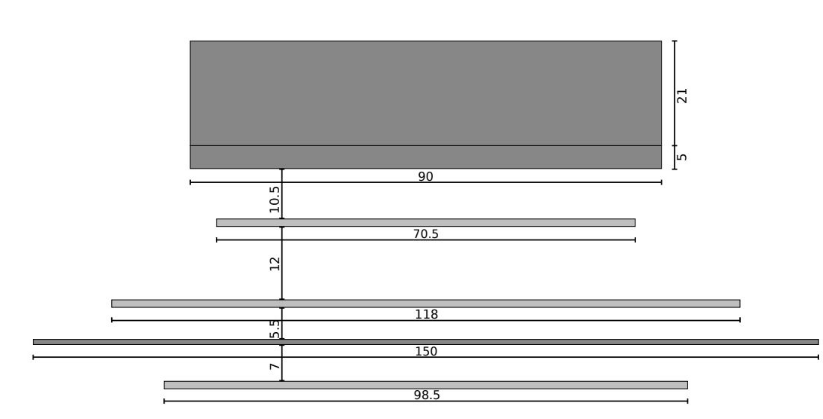
\includegraphics[width=0.63\textwidth]{figures/11.png}
		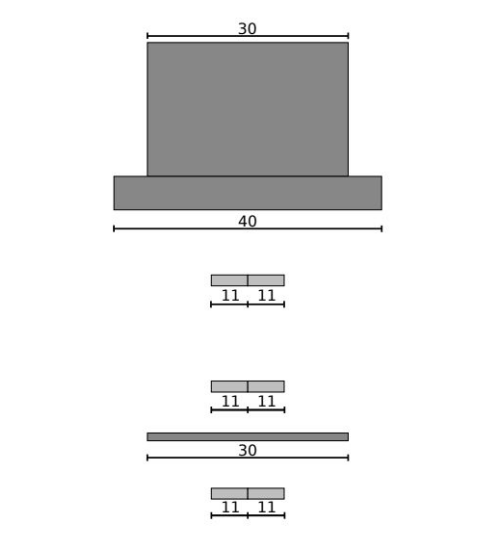
\includegraphics[width=0.36\textwidth]{figures/22.png}
		\caption{The experimental setup where it is shown in lateral and front view the absorber layers (dark grey) and the scintillator planes (light grey) with the dimensions in cm.}
		\label{fig:Scintillators_Detectors}
	\end{figure}
	\begin{figure}
		\centering
		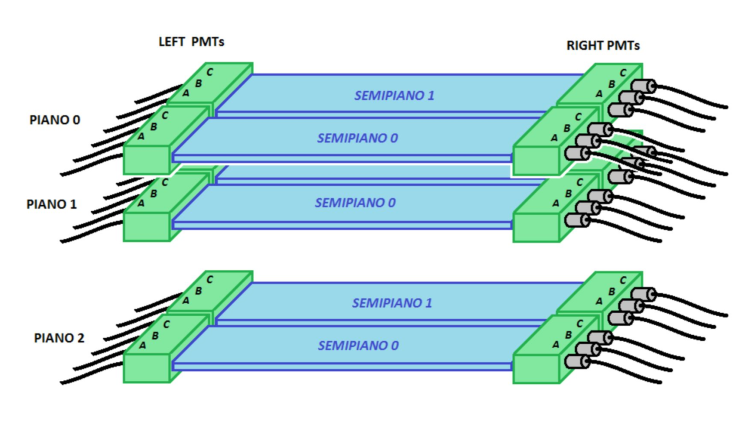
\includegraphics[width=1\textwidth]{figures/33.png}
		\caption{The experimental setup where it is shown in lateral and front view the absorber layers (dark grey) and the scintillator planes (light grey) with the dimensions in cm.}
		\label{fig:Setup}
	\end{figure}
	\vskip 0.09 cm
	Other than the detector itself, we use a NIM (Nuclear Instrument Modules) and a 
    CAMAC (Computer Automated Measurement And Control) crate with appropriate cards and modules.
    All algorithms and tunings of the experiment are done within the NIM crate and CAMAC is used
    for the read-out. The NIM modules which are used can be summarized as follows: 
	\vskip 0.09 cm
	\textbf{HV power supply:}\\ CAEN N470 Quad Channel NIM Programmable High Voltage
    Power Supply ($\pm \SI{8}{kV}, \SI{1}{mA}, \pm \SI{3}{kV}  \SI{3}{mA}$).\\
	This module is the power supply to the photomultiplier tubes. Using the correct functions,
    we can select the channel and set the HV for each PMT.
	\vskip 0.09 cm
	\textbf{Discriminator:}\\ CAEN N840 Octa Channel Leading Edge Discriminator module; pulse width:
    5-40\,ns, and threshold 1-255\,mV.\\
	Given an analog input signal, the discriminator compares the amplitude with a threshold 
    (in mV since it is amplitude). If the falling edge of the input signals overcomes the threshold
    then a LOGIC 1 signal is produced as output. If the signal is lower than the threshold,
    a LOGIC 0 is generated. The Standard LOGIC used by this module is the Nuclear Instrument
    Module Logic (NIM).
	\vskip 0.09 cm
	\textbf{Logic Unit}:\\ CAEN N405 3-fold logic unit module having 3 independent sections to
    perform logic AND/OR up to 4 logic signals in input.\\
	It provides 1 linear OUT (width of the signals depending on input signals superposition),
    2 fixed width (adjustable) OUT signals, 1 ANTI OUT signal, and 1 VETO input.\\
	The first signal enters the LOGIC unit. During this time it is “1” the other signal arrives
    so there is $\Delta t$ during which both signals are “1”. 
    This means the signals coincide and an AND signal is produced.
	\vskip 0.09 cm
	\textbf{FI/FO}:\\ CAEN N625 Quad Linear FAN-IN FAN-OUT module\\
	The module has 4 identical sections. Each section has 4 inputs that can be fed with analog
    signals. Then for each section, there are 4 identical OUT signals. If only one IN is used the
    4 OUT are the replica of the IN signal. If more than one IN is connected then the OUTs provide
    the sum of the IN signals. So each of the 4 sections of this module can be used to replicate 
    a signal 4 times (4 OUT).
	\vskip 0.09 cm
	\textbf{Counter/Scalar:}\\ CAEN N1145 Quad Scaler and Preset Counter/Timer\\
	Count 4 NIM or TTL level signals for a given time interval defined by the user.
    The user can follow the countdown and read the number of counts on displays.

